\chapter*{\center \Large ANEXOS} 
\addcontentsline{toc}{section}{\bfseries ANEXOS} 
\markboth{ANEXOS}{ANEXOS} 

\section*{ANEXO ABET ING 1 - Resolución de problemas}
\addcontentsline{toc}{section}{Resolución de problemas}
Para filtrar por dominio los MAGs obtenidos se evaluaron las siguientes herramientas:

Tiara: Es una herramienta de clasificación de secuencias metagenómicas basada en \textit{deep learning} que permite separar contigs en categorías como arqueas, bacterias, procariotas, eucariotas, orgánulos y secuencias desconocidas mediante un esquema de dos etapas \cite{karlicki2022tiara}. Según su publicación original, mostró un rendimiento similar a EukRep para la clasificación de secuencias procariotas, pero superior para secuencias eucariotas, además de requerir menor tiempo de cómputo \cite{karlicki2022tiara}. Su principal ventaja es que no solo discrimina entre eucariotas y procariotas, sino que también puede identificar ADN organelar, lo que la hace especialmente útil en metagenomas complejos. Sin embargo, al basarse principalmente en patrones de composición de secuencia, puede presentar ambigüedad en linajes evolutivamente inusuales o muy cercanos a eucariotas, por lo que sus resultados deben interpretarse como una clasificación preliminar y no como una asignación taxonómica definitiva.

Whokaryote: Es un clasificador diseñado para distinguir contigs eucariotas y procariotas a partir de características de estructura génica, como la densidad génica, la distancia intergénica y la longitud de los genes, utilizando un modelo de \textit{random forest} \cite{pronk2022whokaryote}. A diferencia de Tiara y EukRep, que dependen sobre todo de frecuencias de \textit{k-mers}, Whokaryote se apoya en diferencias biológicas más interpretables entre ambos dominios. En su artículo, los autores reportan una exactitud cercana al 97\%, indicando además que su desempeño es comparable al de Tiara y EukRep, con la ventaja adicional de aportar una validación independiente basada en otro tipo de señal \cite{pronk2022whokaryote}. Su principal fortaleza es precisamente esa complementariedad metodológica, ya que puede ayudar a confirmar o cuestionar clasificaciones obtenidas por herramientas basadas en composición. Como desventaja, depende de rasgos derivados de genes predichos, por lo que su ejecución es menos directa y puede ser más sensible a la calidad del ensamblado y de la predicción génica subyacente.

EukRep: Es una de las herramientas pioneras para separar secuencias eucariotas de procariotas en ensamblados metagenómicos, utilizando frecuencias de \textit{k-mers} y un clasificador lineal tipo SVM \cite{west2018genomereconstruction}. Su objetivo principal es servir como filtro inicial para recuperar secuencias eucariotas y permitir después el uso de \textit{pipelines} de anotación y análisis específicos para eucariotas. En su publicación original, mostró una exactitud global cercana al 90\% con fragmentos de 3 kb y de aproximadamente 98\% con fragmentos de 20 kb, lo que evidencia un mejor rendimiento en contigs largos \cite{west2018genomereconstruction}. Su ventaja principal es que se trata de una herramienta ampliamente reconocida y adoptada en estudios de recuperación de genomas eucariotas a partir de metagenomas. No obstante, sus limitaciones incluyen un menor desempeño relativo frente a Tiara en la clasificación de eucariotas y la ausencia de una clasificación explícita de secuencias organelares, además de que su precisión puede disminuir en fragmentos más cortos o en ensamblados altamente fragmentados.
\\

\section*{ANEXO ABET ING 5 - Trabajo en equipo}

\addcontentsline{toc}{section}{Trabajo en equipo}
En este anexo se presenta la evidencia del trabajo colaborativo desarrollado durante la ejecución del proyecto. Se podrán incluir reuniones de coordinación, distribución de tareas, seguimiento de avances y productos elaborados en conjunto.

% Agrega aquí tablas, imágenes, capturas o descripciones según tu evidencia.
% Ejemplo:
\begin{figure}[H]
    \centering
    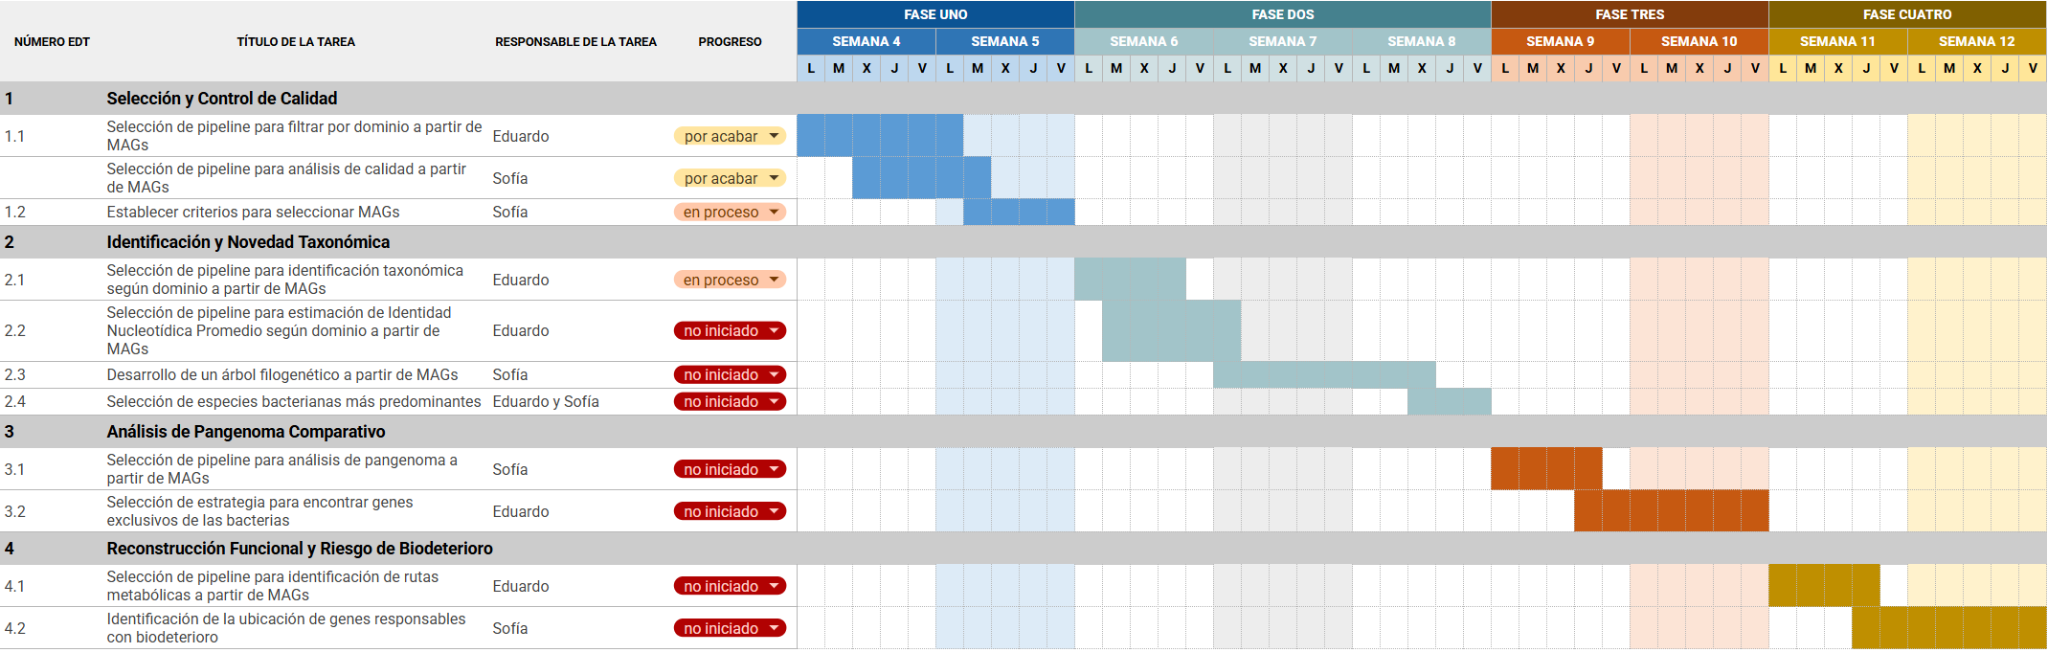
\includegraphics[width=0.8\textwidth]{images/0.png}
    \caption{Diagrama de Gantt del trabajo en equipo durante el desarrollo del proyecto.}
    \label{fig:evidencia_equipo}
\end{figure}


\section*{ANEXO ABET ING 6 --- Experimentación}
\addcontentsline{toc}{section}{Experimentación}
\begin{figure}[H]
    \centering
    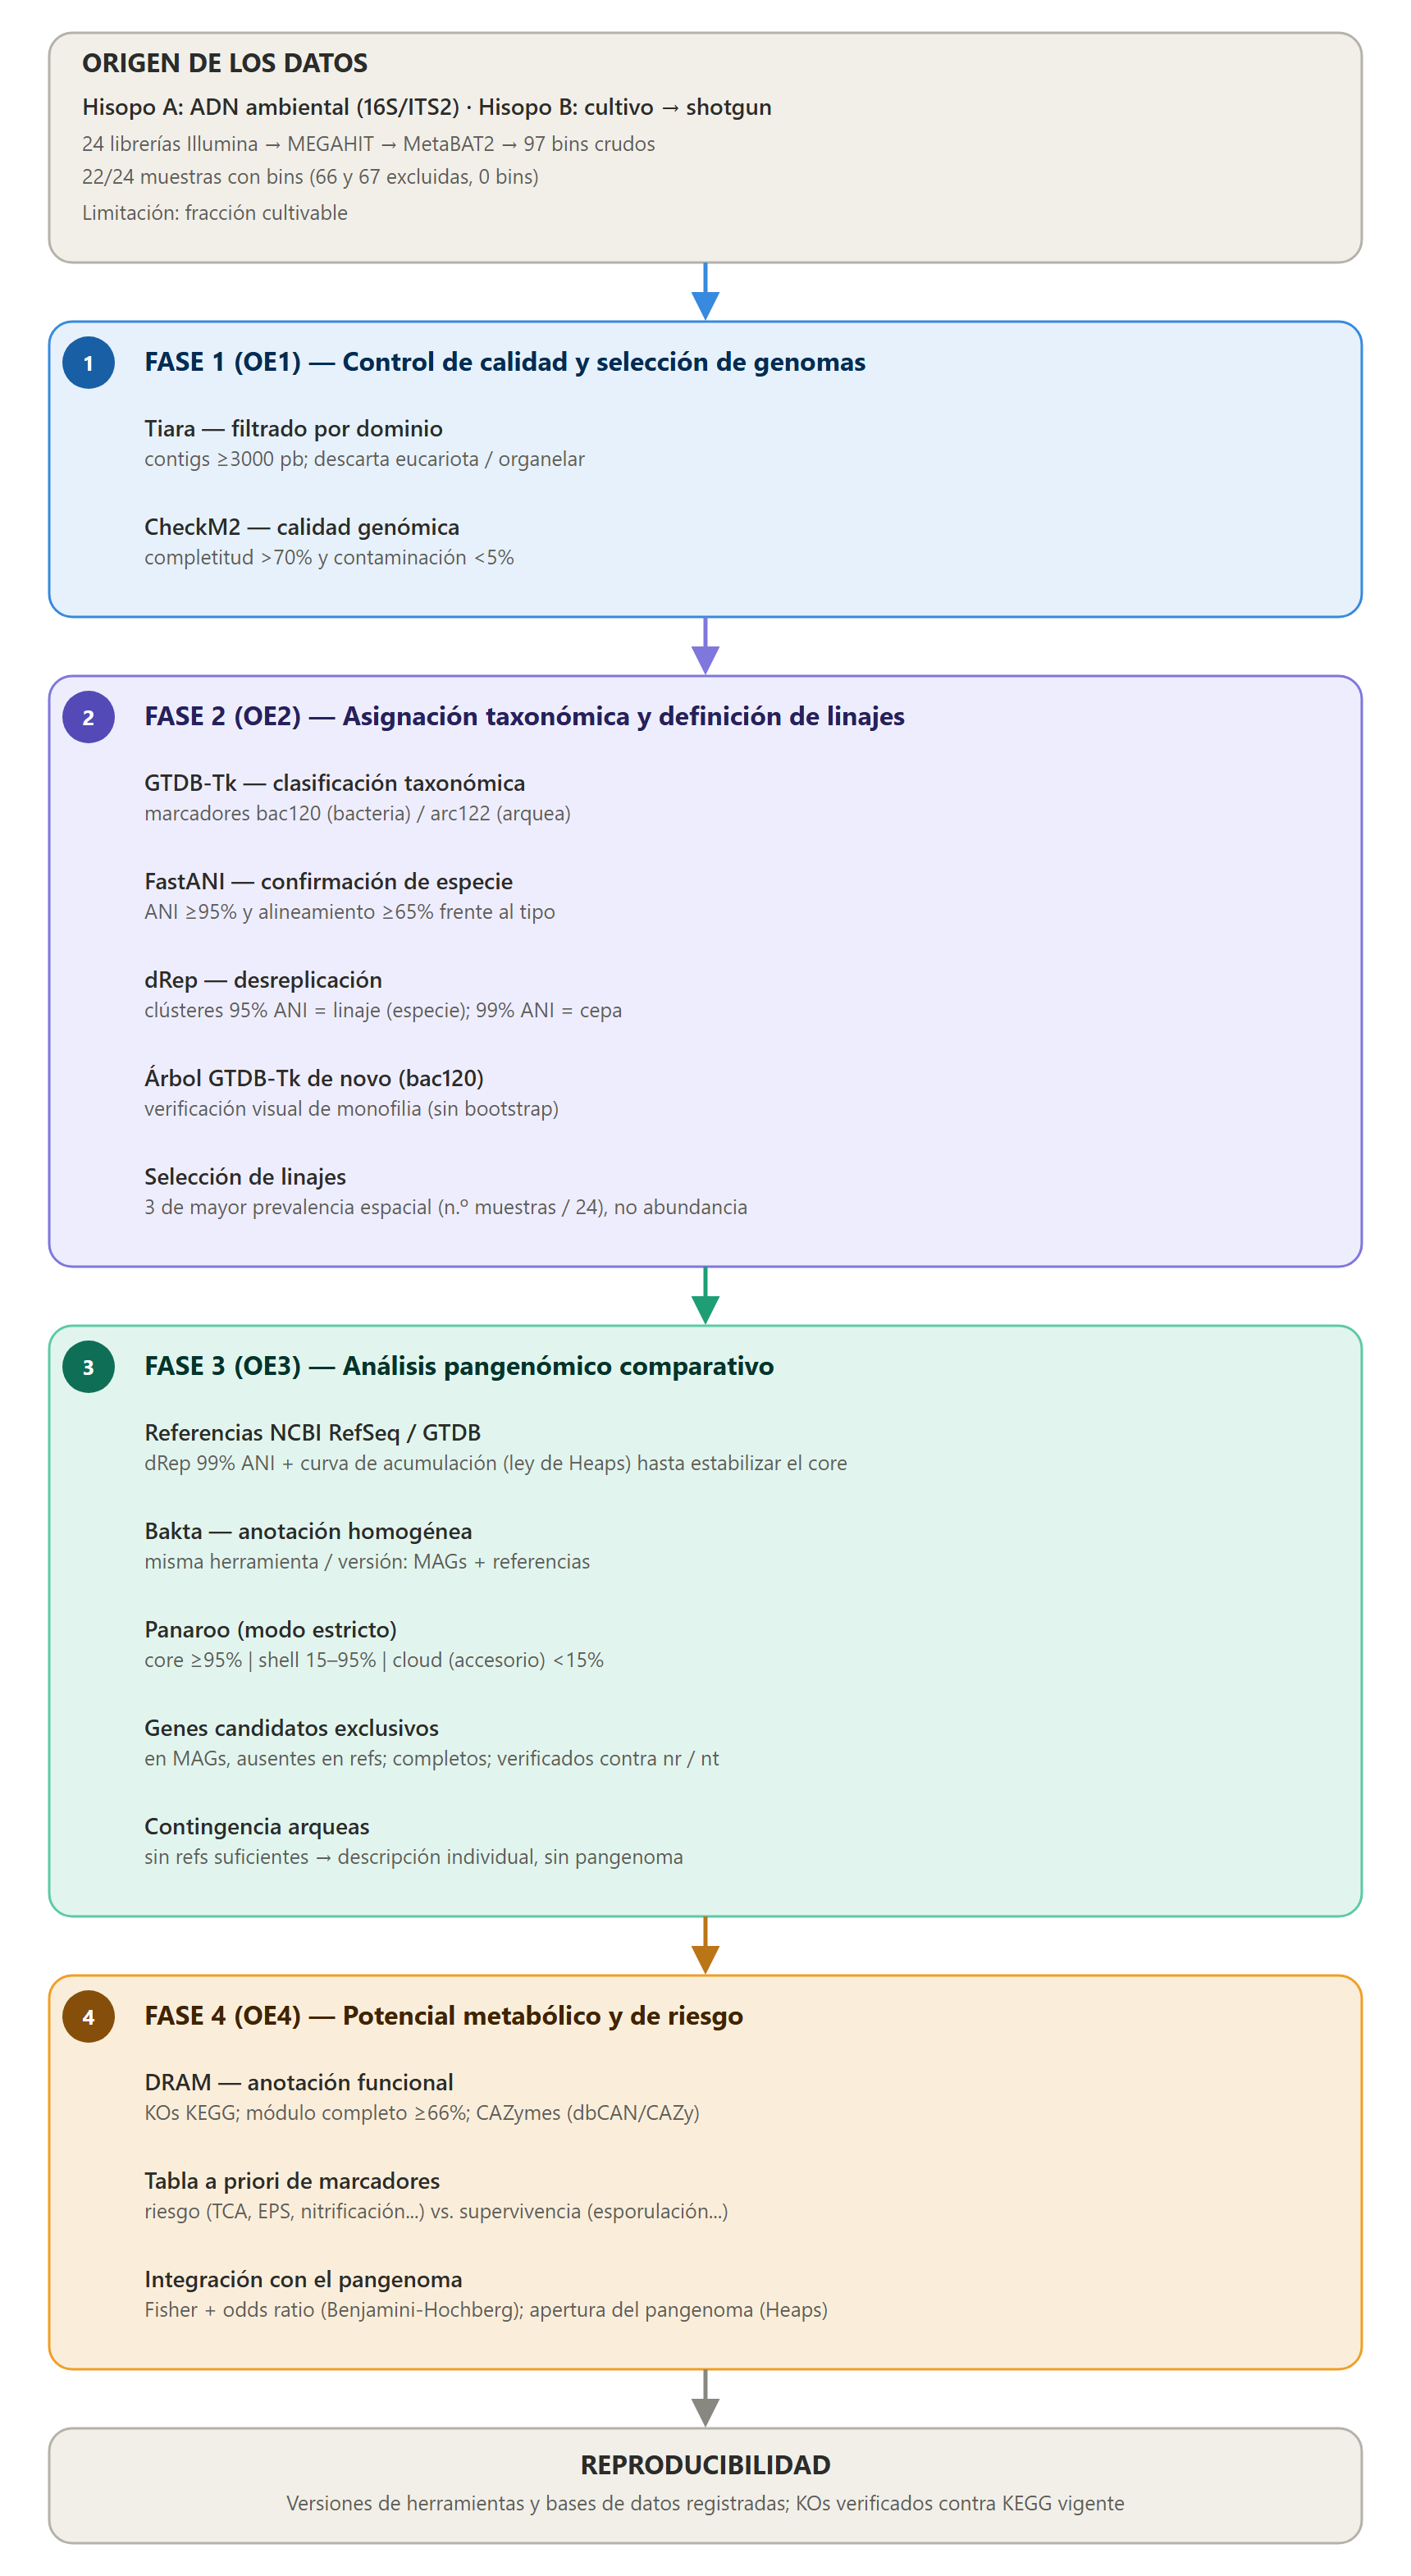
\includegraphics[width=0.8\textwidth]{images/flujograma tesis.png}
    \caption{Flujograma del marco metodológico: cuatro fases consecutivas (OE1 a OE4) desde el origen de los datos metagenómicos hasta la caracterización del potencial metabólico y de riesgo.}
    \label{fig:flujo_metodologico}
\end{figure}


\section*{ANEXO ABET ING 7 --- Aprendizaje continuo}
\addcontentsline{toc}{section}{Aprendizaje continuo}
\renewcommand{\arraystretch}{1.3}
\small
\begin{xltabular}{\textwidth}{|p{1.5cm}|>{\raggedright\arraybackslash}X|>{\raggedright\arraybackslash}p{3cm}|}
\caption{Aprendizaje continuo: fuentes consultadas, contenido aprendido y su aplicación en el documento.}\label{tab:aprendizaje}\\
\hline
\textbf{Ref.} & \textbf{Información o contenido aprendido} & \textbf{Aplicación (en el documento)} \\
\hline
\endfirsthead
\multicolumn{3}{c}{\tablename\ \thetable\ -- continuación}\\
\hline
\textbf{Ref.} & \textbf{Información o contenido aprendido} & \textbf{Aplicación} \\
\hline
\endhead
\hline
\endfoot
\hline
\endlastfoot
~\cite{dakal2012}, ~\cite{li2018deterioration}, ~\cite{chimienti2016}, ~\cite{ding2020preahvihear} & Mecanismos de biodeterioro microbiano de la roca: acidólisis y quelación iónica por ácidos orgánicos de bajo peso molecular, y producción de ácidos nítrico y sulfúrico por bacterias de los ciclos del nitrógeno y del azufre que corroen los minerales. Fundamenta por qué ciertos genes metabólicos implican riesgo material. & Marco Teórico 2.1; Estado del arte; Marco Metodológico \\
\hline
~\cite{villa2016}, ~\cite{PitaGaleana2025}, ~\cite{ding2020}, ~\cite{flemming2010} & Marco ecológico de las biopelículas subaéreas en piedra, arquitectura de la matriz de EPS y rol dual biodeterioro/bioprotección, que motiva pasar de la identidad taxonómica al repertorio funcional. & Formulación del problema; Marco Teórico 2.2; Justificación \\
\hline
~\cite{PitaGaleana2025}, ~\cite{bowers2017} & Flujo de la metagenómica \textit{shotgun}: ensamblaje \textit{de novo} por grafos de De Bruijn y \textit{binning} por composición de tetranucleótidos y cobertura diferencial para reconstruir MAGs. & Formulación del problema; Marco Teórico 2.3; Marco Metodológico\\
\hline
~\cite{checkm2}, ~\cite{bowers2017}, ~\cite{Parks2015} & Definición de completitud y contaminación mediante genes marcadores de copia única; categorías de calidad MIMAG; estimación por aprendizaje automático (CheckM2) sin asignación taxonómica previa. & Marco Teórico 2.4; Marco Metodológico 4.1.3 \\
\hline
~\cite{gtdbtk2019},~\cite{fastANI2018}, ~\cite{gtdb2022}, ~\cite{olm2017} & Clasificación genómica normalizada por divergencia evolutiva (GTDB-Tk/GTDB), delimitación de especie por ANI (umbral del 95\%) y sdereplicación para colapsar genomas redundantes y definir linajes. & Marco Teórico 2.5; Marco Metodológico 4.1.4 \\
\hline
~\cite{panaroo2020},~\cite{tettelin2005} & Concepto de pangenoma y partición en genoma núcleo, cubierta y accesorio; la transferencia horizontal como motor de adaptación; corrección de la inflación del accesorio por fragmentación mediante grafos (Panaroo). & Marco Teórico 2.6; Marco Metodológico 4.1.5 \\
\hline
~\cite{dram2020},~\cite{Hyatt2010}, ~\cite{schwengers2021} & Predicción de ORFs y anotación estandarizada sin alineamiento (Bakta); destilación del metabolismo y cálculo de completitud de módulos/rutas (DRAM) sobre ortólogos KEGG, base para inferir el potencial de biodeterioro. & Marco Teórico 2.7; Marco Metodológico 4.1.6 \\
\hline
~\cite{karlicki2022tiara},~\cite{pronk2022whokaryote}, ~\cite{west2018genomereconstruction} & Clasificadores de contigs por dominio: aprendizaje profundo sobre composición (Tiara), estructura génica con \textit{random forest} (Whokaryote) y \textit{k-mers} con SVM (EukRep); criterios para seleccionar la herramienta de filtrado. & Marco Metodológico 4.1.3.1; Anexo 1 \\
\hline
~\cite{cordycollins1993},~\cite{hernandez2012}, ~\cite{mnaahp2015} & Contexto histórico-arqueológico de la Estela de Raimondi: filiación con la cultura Chavín, hallazgo, traslados sucesivos y custodia museística actual. & Introducción (Presentación del proyecto) \\
\hline
\end{xltabular}

\section{Anexo: Repositorio de GitHub}

Link: \href{https://github.com/EduardoTllo/biodeterioro-estela-pipeline}{GitHub}

\section{Anexo: Reporte completo de calidad y selección de bins (Fase 1)}
\label{anexo:tabla_completa_bins}

\begingroup
\small
\setlength{\tabcolsep}{2.5pt} % Espaciado entre columnas

\begin{xltabular}{\textwidth}{|c|c|c|c|c|c|>{\centering\arraybackslash}X|}
\caption{Reporte completo de evaluación y filtrado de bins genómicos (Fase 1).} \label{anexo:tabla_completa_bins} \\
\hline
\textbf{Bin} & \textbf{Contigs} & \textbf{Long (bp)} & \textbf{Dom.} & \textbf{Comp. (\%)} & \textbf{Contam. (\%)} & \textbf{Motivo} \\
\hline
\endfirsthead

\multicolumn{7}{c}{{\bfseries \tablename\ \thetable{} -- Continuación de la página anterior}} \\
\hline
\textbf{Bin} & \textbf{Contigs} & \textbf{Long (bp)} & \textbf{Dom.} & \textbf{Comp. (\%)} & \textbf{Contam. (\%)} & \textbf{Motivo} \\
\hline
\endhead

\hline
\multicolumn{7}{r}{{Continúa en la siguiente página...}} \\
\hline
\endfoot

\hline
\endlastfoot

bin-1-49 & 87 & 545.053 & euk & -- & -- & dominio mayoritario: euk \\ \hline
bin-1-50 & 224 & 2.609.893 & prok & 62.29 & 2.66 & completitud 62.29 $\le$ 70 \\ \hline
bin-1-51 & 51 & 4.727.435 & prok & 100.00 & 0.00 & - \\ \hline
bin-1-52 & 26 & 415.732 & prok & 6.05 & 0.20 & completitud 6.05 $\le$ 70 \\ \hline
bin-1-53 & 30 & 2.476.631 & prok & 99.84 & 0.12 & - \\ \hline
bin-1-54 & 49 & 4.312.038 & prok & 92.25 & 0.01 & - \\ \hline
bin-1-55 & 247 & 34.242.081 & euk & -- & -- & dominio mayoritario: euk \\ \hline
bin-1-56 & 12 & 230.366 & euk & -- & -- & dominio mayoritario: euk \\ \hline
bin-1-57 & 22 & 4.032.412 & prok & 99.99 & 3.23 & - \\ \hline
bin-1-58 & 4725 & 12.125.594 & unknown & 0.00 & 17.71 & completitud 0.00 $\le$ 70; contaminacion 17.71 $\ge$ 5 \\ \hline
bin-1-59 & 98 & 5.907.869 & prok & 99.97 & 3.07 & - \\ \hline
bin-1-60 & 302 & 8.273.570 & prok & 100.00 & 24.87 & contaminacion 24.87 $\ge$ 5 \\ \hline
bin-1-61 & 448 & 40.131.343 & euk & -- & -- & dominio mayoritario: euk \\ \hline
bin-1-62 & 320 & 7.390.811 & prok & 99.72 & 72.67 & contaminacion 72.67 $\ge$ 5 \\ \hline
bin-1-63 & 162 & 65.185.746 & prok & 84.85 & 39.63 & contaminacion 39.63 $\ge$ 5 \\ \hline
bin-1-64 & 163 & 3.944.265 & prok & 99.84 & 0.59 & - \\ \hline
bin-1-65 & 322 & 29.636.962 & euk & -- & -- & dominio mayoritario: euk \\ \hline
bin-1-68 & 50 & 2.465.224 & prok & 100.00 & 1.79 & - \\ \hline
bin-1-69 & 67 & 251.086 & prok & 6.60 & 0.14 & completitud 6.60 $\le$ 70 \\ \hline
bin-1-70 & 3805 & 494.251.631 & unknown & 31.70 & 28.68 & completitud 31.70 $\le$ 70; contaminacion 28.68 $\ge$ 5 \\ \hline
bin-1-71 & 37 & 11.498.934 & prok & 67.71 & 15.05 & completitud 67.71 $\le$ 70; contaminacion 15.05 $\ge$ 5 \\ \hline
bin-1-72 & 16 & 7.408.652 & unknown & 5.87 & 0.19 & completitud 5.87 $\le$ 70 \\ \hline
bin-10-71 & 506 & 2.845.557 & prok & 97.57 & 30.13 & contaminacion 30.13 $\ge$ 5 \\ \hline
bin-11-71 & 4161 & 101.946.556 & unknown & 65.68 & 17.72 & completitud 65.68 $\le$ 70; contaminacion 17.72 $\ge$ 5 \\ \hline
bin-12-71 & 383 & 1.015.904 & unknown & 43.42 & 3.52 & completitud 43.42 $\le$ 70 \\ \hline
bin-2-49 & 134 & 27.557.437 & euk & -- & -- & dominio mayoritario: euk \\ \hline
bin-2-50 & 464 & 53.406.620 & euk & -- & -- & dominio mayoritario: euk \\ \hline
bin-2-52 & 270 & 5.347.688 & prok & 99.93 & 8.10 & contaminacion 8.10 $\ge$ 5 \\ \hline
bin-2-53 & 39 & 5.164.804 & prok & 99.99 & 0.57 & - \\ \hline
bin-2-54 & 106 & 7.273.841 & prok & 100.00 & 15.52 & contaminacion 15.52 $\ge$ 5 \\ \hline
bin-2-56 & 816 & 49.647.189 & euk & -- & -- & dominio mayoritario: euk \\ \hline
bin-2-57 & 28 & 5.172.263 & prok & 99.96 & 1.01 & - \\ \hline
bin-2-58 & 17 & 4.771.531 & prok & 100.00 & 0.06 & - \\ \hline
bin-2-59 & 424 & 23.212.147 & prok & 91.94 & 115.89 & contaminacion 115.89 $\ge$ 5 \\ \hline
bin-2-60 & 290 & 10.390.751 & prok & 100.00 & 100.33 & contaminacion 100.33 $\ge$ 5 \\ \hline
bin-2-61 & 9 & 614.253 & euk & -- & -- & dominio mayoritario: euk \\ \hline
bin-2-62 & 5 & 227.679 & euk & -- & -- & dominio mayoritario: euk \\ \hline
bin-2-63 & 150 & 4.282.638 & prok & 92.39 & 0.34 & - \\ \hline
bin-2-64 & 924 & 226.083.286 & unknown & 0.02 & 16.03 & completitud 0.02 $\le$ 70; contaminacion 16.03 $\ge$ 5 \\ \hline
bin-2-65 & 141 & 17.056.380 & euk & -- & -- & dominio mayoritario: euk \\ \hline
bin-2-68 & 70 & 246.182 & prok & 4.99 & 0.03 & completitud 4.99 $\le$ 70 \\ \hline
bin-2-69 & 61 & 2.481.071 & prok & 99.99 & 0.18 & - \\ \hline
bin-2-70 & 87 & 278.635 & unknown & 5.38 & 0.09 & completitud 5.38 $\le$ 70 \\ \hline
bin-2-71 & 618 & 1.368.774 & unknown & 56.83 & 26.01 & completitud 56.83 $\le$ 70; contaminacion 26.01 $\ge$ 5 \\ \hline
bin-2-72 & 667 & 2.485.725 & prok & 79.16 & 54.30 & contaminacion 54.30 $\ge$ 5 \\ \hline
bin-3-50 & 30 & 2.607.902 & unknown & 13.03 & 0.08 & completitud 13.03 $\le$ 70 \\ \hline
bin-3-52 & 204 & 5.184.467 & prok & 98.97 & 0.58 & - \\ \hline
bin-3-53 & 301 & 29.244.092 & euk & -- & -- & dominio mayoritario: euk \\ \hline
bin-3-56 & 160 & 26.628.065 & euk & -- & -- & dominio mayoritario: euk \\ \hline
bin-3-57 & 818 & 25.745.728 & euk & -- & -- & dominio mayoritario: euk \\ \hline
bin-3-58 & 265 & 29.647.785 & euk & -- & -- & dominio mayoritario: euk \\ \hline
bin-3-60 & 959 & 2.321.293 & unknown & 39.27 & 0.00 & completitud 39.27 $\le$ 70 \\ \hline
bin-3-61 & 50 & 10.715.439 & euk & -- & -- & dominio mayoritario: euk \\ \hline
bin-3-62 & 117 & 449.659 & euk & -- & -- & dominio mayoritario: euk \\ \hline
bin-3-63 & 4589 & 19.740.558 & prok & 99.91 & 102.18 & contaminacion 102.18 $\ge$ 5 \\ \hline
bin-3-64 & 459 & 2.352.198 & prok & 70.14 & 0.64 & - \\ \hline
bin-3-65 & 5256 & 27.711.612 & euk & -- & -- & dominio mayoritario: euk \\ \hline
bin-3-70 & 169 & 64.261.799 & unknown & 77.48 & 75.48 & contaminacion 75.48 $\ge$ 5 \\ \hline
bin-3-71 & 3657 & 12.324.162 & prok & 97.39 & 70.70 & contaminacion 70.70 $\ge$ 5 \\ \hline
bin-3-72 & 174 & 16.597.747 & prok & 98.53 & 98.35 & contaminacion 98.35 $\ge$ 5 \\ \hline
bin-4-50 & 97 & 1.654.013 & prok & 43.00 & 0.23 & completitud 43.00 $\le$ 70 \\ \hline
bin-4-52 & 96 & 3.497.259 & prok & 99.86 & 0.25 & - \\ \hline
bin-4-56 & 122 & 1.739.035 & euk & -- & -- & dominio mayoritario: euk \\ \hline
bin-4-57 & 977 & 39.075.173 & euk & -- & -- & dominio mayoritario: euk \\ \hline
bin-4-60 & 4482 & 25.724.799 & euk & -- & -- & dominio mayoritario: euk \\ \hline
bin-4-61 & 1610 & 11.012.084 & prok & 100.00 & 58.51 & contaminacion 58.51 $\ge$ 5 \\ \hline
bin-4-62 & 270 & 79.759.046 & prok & 90.25 & 65.70 & contaminacion 65.70 $\ge$ 5 \\ \hline
bin-4-63 & 856 & 56.508.797 & euk & -- & -- & dominio mayoritario: euk \\ \hline
bin-4-64 & 428 & 29.693.972 & euk & -- & -- & dominio mayoritario: euk \\ \hline
bin-4-65 & 2506 & 20.150.702 & prok & 99.99 & 106.28 & contaminacion 106.28 $\ge$ 5 \\ \hline
bin-4-70 & 484 & 1.565.460 & prok & 64.00 & 2.55 & completitud 64.00 $\le$ 70 \\ \hline
bin-4-71 & 216 & 488.562 & unknown & 32.24 & 2.32 & completitud 32.24 $\le$ 70 \\ \hline
bin-4-72 & 72 & 248.801 & prok & 4.69 & 0.01 & completitud 4.69 $\le$ 70 \\ \hline
bin-5-50 & 1041 & 3.472.002 & prok & 76.56 & 0.44 & - \\ \hline
bin-5-52 & 1099 & 3.740.736 & prok & 95.51 & 12.95 & contaminacion 12.95 $\ge$ 5 \\ \hline
bin-5-56 & 146 & 552.204 & euk & -- & -- & dominio mayoritario: euk \\ \hline
bin-5-57 & 12 & 224.138 & euk & -- & -- & dominio mayoritario: euk \\ \hline
bin-5-60 & 97 & 2.849.856 & prok & 77.53 & 0.10 & - \\ \hline
bin-5-61 & 273 & 5.811.268 & prok & 97.82 & 10.64 & contaminacion 10.64 $\ge$ 5 \\ \hline
bin-5-62 & 222 & 27.886.446 & euk & -- & -- & dominio mayoritario: euk \\ \hline
bin-5-63 & 90 & 2.758.939 & prok & 72.46 & 0.05 & - \\ \hline
bin-5-64 & 217 & 39.450.268 & prok & 100.00 & 67.99 & contaminacion 67.99 $\ge$ 5 \\ \hline
bin-5-65 & 24 & 222.213 & euk & -- & -- & dominio mayoritario: euk \\ \hline
bin-5-70 & 28 & 2.628.283 & unknown & 48.48 & 2.40 & completitud 48.48 $\le$ 70 \\ \hline
bin-5-71 & 118 & 438.388 & prok & 12.74 & 0.54 & completitud 12.74 $\le$ 70 \\ \hline
bin-6-50 & 591 & 5.543.214 & prok & 100.00 & 0.65 & - \\ \hline
bin-6-56 & 116 & 9.578.458 & euk & -- & -- & dominio mayoritario: euk \\ \hline
bin-6-57 & 126 & 448.524 & euk & -- & -- & dominio mayoritario: euk \\ \hline
bin-6-61 & 30 & 4.792.746 & prok & 100.00 & 0.74 & - \\ \hline
bin-6-63 & 21 & 367.167 & euk & -- & -- & dominio mayoritario: euk \\ \hline
bin-6-64 & 71 & 239.057 & euk & -- & -- & dominio mayoritario: euk \\ \hline
bin-6-70 & 319 & 48.190.971 & unknown & 68.24 & 17.99 & completitud 68.24 $\le$ 70; contaminacion 17.99 $\ge$ 5 \\ \hline
bin-6-71 & 34 & 453.921 & prok & 11.79 & 0.16 & completitud 11.79 $\le$ 70 \\ \hline
bin-7-64 & 1246 & 3.769.741 & prok & 60.17 & 0.22 & completitud 60.17 $\le$ 70 \\ \hline
bin-7-71 & 95 & 258.968 & unknown & 7.21 & 0.05 & completitud 7.21 $\le$ 70 \\ \hline
bin-8-71 & 908 & 2.450.575 & unknown & 81.92 & 35.87 & contaminacion 35.87 $\ge$ 5 \\ \hline
bin-9-71 & 346 & 1.832.072 & prok & 85.09 & 2.13 & - \\
\end{xltabular}
\endgroup